
\pdfminorversion=4 % for acroread
\documentclass[aspectratio=169,t,xcolor={usenames,dvipsnames}]{beamer}
%\documentclass[t,handout,xcolor={usenames,dvipsnames}]{beamer}
\usepackage{../beamerstyle}
\usepackage{dsfont}
\usepackage{bm}
\usepackage[english]{babel}
\usepackage[utf8]{inputenc}
\usepackage{graphicx}
\usepackage{algorithm}
\usepackage[ruled,vlined,algo2e,linesnumbered]{algorithm2e}
%\usepackage[boxed,vlined]{algorithm2e}
\usepackage{hyperref}
\usepackage{booktabs}
\usepackage{mathtools}

\usepackage{amsmath,amssymb}
\usepackage{listings}
\lstset{frame=lines,framesep=3pt,numbers=left,numberblanklines=false,basicstyle=\ttfamily\small}

\usepackage{subfig}
\usepackage{multicol}
%\usepackage{appendixnumberbeamer}
%
\usepackage{tcolorbox}

\usepackage{pgfplots}
\usepackage{tikz}
\usetikzlibrary{trees} 
\usetikzlibrary{shapes.geometric}
\usetikzlibrary{positioning,shapes,shadows,arrows,calc,mindmap}
\usetikzlibrary{positioning,fadings,through}
\usetikzlibrary{decorations.pathreplacing}
\usetikzlibrary{intersections}
\usetikzlibrary{positioning,fit,calc,shadows,backgrounds}
\pgfdeclarelayer{background}
\pgfdeclarelayer{foreground}
\pgfsetlayers{background,main,foreground}
\tikzstyle{activity}=[rectangle, draw=black, rounded corners, text centered, text width=8em]
\tikzstyle{data}=[rectangle, draw=black, text centered, text width=8em]
\tikzstyle{myarrow}=[->, thick, draw=black]

% Define the layers to draw the diagram
\pgfdeclarelayer{background}
\pgfdeclarelayer{foreground}
\pgfsetlayers{background,main,foreground}

%\usepackage{listings}
%\lstset{numbers=left,
%  showstringspaces=false,
%  frame={tb},
%  captionpos=b,
%  lineskip=0pt,
%  basicstyle=\ttfamily,
%%  extendedchars=true,
%  stepnumber=1,
%  numberstyle=\small,
%  xleftmargin=1em,
%  breaklines
%}

 
\definecolor{blue}{RGB}{0, 74, 153}

\usetheme{Boadilla}
%\useinnertheme{rectangles}
\usecolortheme{whale}
\setbeamercolor{alerted text}{fg=blue}
\useoutertheme{infolines}
\setbeamertemplate{navigation symbols}{\vspace{-5pt}} % to lower the logo
\setbeamercolor{date in head/foot}{bg=blue} % blue
\setbeamercolor{date in head/foot}{fg=white}
\setbeamercolor{author in head/foot}{bg=blue} %blue
\setbeamercolor{title in head/foot}{bg=blue} % blue
\setbeamercolor{title}{fg=white, bg=blue}
\setbeamercolor{block title}{fg=white,bg=blue}
\setbeamercolor{block body}{bg=blue!10}
\setbeamercolor{frametitle}{fg=white, bg=blue}
\setbeamercovered{invisible}

\makeatletter
\setbeamertemplate{footline}
{
  \leavevmode%
  \hbox{%
  \begin{beamercolorbox}[wd=.333333\paperwidth,ht=2.25ex,dp=1ex,center]{author in head/foot}%
    \usebeamerfont{author in head/foot}\insertshortauthor
  \end{beamercolorbox}%
  \begin{beamercolorbox}[wd=.333333\paperwidth,ht=2.25ex,dp=1ex,center]{title in head/foot}%
    \usebeamerfont{title in head/foot}\insertshorttitle
  \end{beamercolorbox}%
  \begin{beamercolorbox}[wd=.333333\paperwidth,ht=2.25ex,dp=1ex,right]{date in head/foot}%
    \usebeamerfont{date in head/foot}Week \@week, Topic \@topicnumber, Slide \insertframenumber{}\hspace*{2em}
%    \insertframenumber\hspace*{2ex} 
  \end{beamercolorbox}}%
  \vskip0pt%
}

\newcommand{\@week}{0}
\newcommand{\@topicnumber}{0}
\newcommand{\week}[1]{\renewcommand{\@week}{#1}}
\newcommand{\topicnumber}[1]{\renewcommand{\@topicnumber}{#1}}

\makeatother

%\pgfdeclareimage[height=1.2cm]{automl}{images/logos/automl.png}
%\pgfdeclareimage[height=1.2cm]{freiburg}{images/logos/freiburg}

%\logo{\pgfuseimage{freiburg}}

\input{../latex_main/macros}





\title[AutoML: Overview]{AutoML: Algorithm Selection} % week title
\subtitle{Features} % video title
\author[Lars Kotthoff]{Bernd Bischl \and Frank Hutter \and \underline{Lars Kotthoff}\newline \and Marius Lindauer \and Joaquin Vanschoren}
\institute{}
\date{}
\week{3}
\topicnumber{3}


% \AtBeginSection[] % Do nothing for \section*
% {
%   \begin{frame}{Outline}
%     \bigskip
%     \vfill
%     \tableofcontents[currentsection]
%   \end{frame}
% }

\begin{document}
	
\maketitle

\begin{frame}[c]{Algorithm Selection}
\begin{center}
\resizebox{.7\textwidth}{!}{%
\tikzset{>=latex}
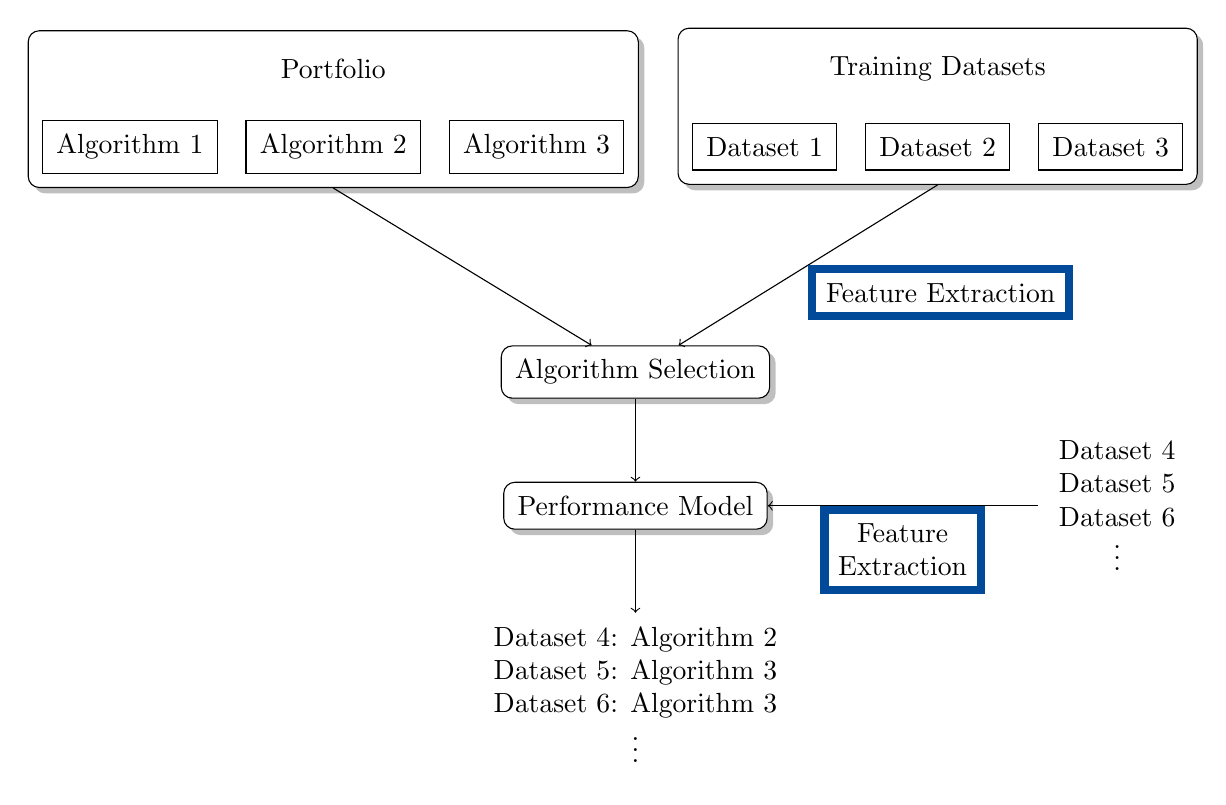
\begin{tikzpicture}[node distance=1em,inner sep=.5em,n/.style={drop
shadow,fill=white,rounded corners},scale=.5]
\node (p) [align=left] {Portfolio};
\node (a2) [rectangle,align=center,below=of p,draw] {Algorithm 2};
\node (a1) [rectangle,align=center,left=of a2,draw] {Algorithm 1};
\node (a3) [rectangle,align=center,right=of a2,draw] {Algorithm 3};
\begin{pgfonlayer}{background}
\node (pc) [n,fit={(p) (a1) (a2) (a3)},draw] {};
\end{pgfonlayer}

\node (i) [align=left,right=15em of p.east] {Training Datasets};
\node (i2) [rectangle,align=center,below=of i,draw] {Dataset 2};
\node (i1) [rectangle,align=center,left=of i2,draw] {Dataset 1};
\node (i3) [rectangle,align=center,right=of i2,draw] {Dataset 3};
\begin{pgfonlayer}{background}
\node (ic) [n,fit={(i) (i1) (i2) (i3)},draw] {};
\end{pgfonlayer}

\node (as) [n,draw,align=left,below=10em of $(p)!0.5!(i)$] {Algorithm Selection};
\node (m) [n,draw,align=left,below=3em of as] {Performance Model};

\node (it) [align=center,right=10em of m] {Dataset 4\\Dataset 5\\Dataset 6\\$\vdots$};

\node (s) [align=center,below=3em of m] {Dataset 4: Algorithm 2\\Dataset 5: Algorithm 3\\Dataset 6: Algorithm 3\\$\vdots$};

\path [->] (pc.south) edge (as);
\path [->] (ic.south) edge node [below right, rectangle, draw = blue, line width = 3pt] {Feature Extraction} (as);
\path [->] ([xshift=-.5em]it.west) edge node [below,align=center, rectangle, draw = blue, line width = 3pt] {Feature\\Extraction} (m.east);
\path [->] (as.south) edge (m.north);
\path [->] (m.south) edge (s.north);
\end{tikzpicture}}
\end{center}
\end{frame}

\begin{frame}[c]{Features}
\begin{itemize}
\item relate properties of datasets to algorithm performance
\item relatively cheap to compute -- must be cheaper than running the algorithm
    to see what its performance is
\item often specified by domain expert
\item syntactic and information-theoretic -- analyze dataset
\item probing -- run an algorithm for short time or on subset of data
\end{itemize}
\end{frame}

\begin{frame}[c]{Syntactic and Information-Theoretic Features}
    \begin{itemize}
        \item number of binary/numeric/categorical features
        \item number of classes
        \item class entropy
        \item skewness of classes
        \item fraction of missing values
        \item correlation between features and target
        \item \ldots
    \end{itemize}
\end{frame}

\begin{frame}[c]{Probing Features (Landmarkers)}
    \begin{itemize}
        \item performance of majority class/mean value predictor
        \item decision stump performance
        \item simple rule model performance
        \item performance of algorithm of interest on 1\% of data
        \item \ldots
    \end{itemize}
    $\rightarrow$ usually leads to much better results that using just syntactic
    and information-theoretic features
\end{frame}

\begin{frame}[c]{No Features}
    \begin{itemize}
        \item use deep learning to process dataset or problem instance as-is
        \item no need for expert-designed features
        \item only preliminary applications so far, performance not good, no widespread adoption yet
    \end{itemize}
\end{frame}

\begin{frame}[c]{Aside: Algorithm Features}
    \begin{itemize}
        \item can characterize algorithm in addition to datasets
        \item allows to relate performance to specific aspects of an algorithm
            rather than black boxes
        \item for example size of code base, properties of abstract syntax
            tree\ldots
        \item ongoing work
    \end{itemize}
\end{frame}

\begin{frame}[c]{What Features Do We Need in Practice?}
    \begin{itemize}
        \item trade-off between complex features and complex models
        \item in practice, very simple features can perform well
        \item often only few features of a set are needed (e.g.\ 5 out of $>$100)
        \item in the end, whatever works best
    \end{itemize}
\end{frame}

\end{document}
